\documentclass[10pt, spanish]{article}
\usepackage[spanish]{babel}
\selectlanguage{spanish}
\usepackage{natbib}
\usepackage{url}
\usepackage[utf8x]{inputenc}
\usepackage{graphicx}
\graphicspath{{images/}}
\usepackage{parskip}
\usepackage{fancyhdr}
\usepackage{vmargin}
\usepackage{multirow}
\usepackage{float}
\usepackage{chngpage}

\usepackage{subcaption}

\usepackage{hyperref}
\usepackage[
    type={CC},
    modifier={by-nc-sa},
    version={4.0},
]{doclicense}

\hypersetup{
    colorlinks=true,
    linkcolor=blue,
    filecolor=magenta,      
    urlcolor=cyan,
}

% para codigo
\usepackage{listings}
\usepackage{xcolor}



%% configuración de listings

\definecolor{listing-background}{HTML}{F7F7F7}
\definecolor{listing-rule}{HTML}{B3B2B3}
\definecolor{listing-numbers}{HTML}{B3B2B3}
\definecolor{listing-text-color}{HTML}{000000}
\definecolor{listing-keyword}{HTML}{435489}
\definecolor{listing-identifier}{HTML}{435489}
\definecolor{listing-string}{HTML}{00999A}
\definecolor{listing-comment}{HTML}{8E8E8E}
\definecolor{listing-javadoc-comment}{HTML}{006CA9}

\lstdefinestyle{eisvogel_listing_style}{
  language         = c++,
%$if(listings-disable-line-numbers)$
%  xleftmargin      = 0.6em,
%  framexleftmargin = 0.4em,
%$else$
  numbers          = left,
  xleftmargin      = 0em,
 framexleftmargin = 0em,
%$endif$
  backgroundcolor  = \color{listing-background},
  basicstyle       = \color{listing-text-color}\small\ttfamily{}\linespread{1.15}, % print whole listing small
  breaklines       = true,
  frame            = single,
  framesep         = 0.19em,
  rulecolor        = \color{listing-rule},
  frameround       = ffff,
  tabsize          = 4,
  numberstyle      = \color{listing-numbers},
  aboveskip        = 1.0em,
  belowskip        = 0.1em,
  abovecaptionskip = 0em,
  belowcaptionskip = 1.0em,
  keywordstyle     = \color{listing-keyword}\bfseries,
  classoffset      = 0,
  sensitive        = true,
  identifierstyle  = \color{listing-identifier},
  commentstyle     = \color{listing-comment},
  morecomment      = [s][\color{listing-javadoc-comment}]{/**}{*/},
  stringstyle      = \color{listing-string},
  showstringspaces = false,
  escapeinside     = {/*@}{@*/}, % Allow LaTeX inside these special comments
  literate         =
  {á}{{\'a}}1 {é}{{\'e}}1 {í}{{\'i}}1 {ó}{{\'o}}1 {ú}{{\'u}}1
  {Á}{{\'A}}1 {É}{{\'E}}1 {Í}{{\'I}}1 {Ó}{{\'O}}1 {Ú}{{\'U}}1
  {à}{{\`a}}1 {è}{{\'e}}1 {ì}{{\`i}}1 {ò}{{\`o}}1 {ù}{{\`u}}1
  {À}{{\`A}}1 {È}{{\'E}}1 {Ì}{{\`I}}1 {Ò}{{\`O}}1 {Ù}{{\`U}}1
  {ä}{{\"a}}1 {ë}{{\"e}}1 {ï}{{\"i}}1 {ö}{{\"o}}1 {ü}{{\"u}}1
  {Ä}{{\"A}}1 {Ë}{{\"E}}1 {Ï}{{\"I}}1 {Ö}{{\"O}}1 {Ü}{{\"U}}1
  {â}{{\^a}}1 {ê}{{\^e}}1 {î}{{\^i}}1 {ô}{{\^o}}1 {û}{{\^u}}1
  {Â}{{\^A}}1 {Ê}{{\^E}}1 {Î}{{\^I}}1 {Ô}{{\^O}}1 {Û}{{\^U}}1
  {œ}{{\oe}}1 {Œ}{{\OE}}1 {æ}{{\ae}}1 {Æ}{{\AE}}1 {ß}{{\ss}}1
  {ç}{{\c c}}1 {Ç}{{\c C}}1 {ø}{{\o}}1 {å}{{\r a}}1 {Å}{{\r A}}1
  {€}{{\EUR}}1 {£}{{\pounds}}1 {«}{{\guillemotleft}}1
  {»}{{\guillemotright}}1 {ñ}{{\~n}}1 {Ñ}{{\~N}}1 {¿}{{?`}}1
  {…}{{\ldots}}1 {≥}{{>=}}1 {≤}{{<=}}1 {„}{{\glqq}}1 {“}{{\grqq}}1
  {”}{{''}}1
}
\lstset{style=eisvogel_listing_style}


\usepackage[default]{sourcesanspro}

\setmarginsrb{2 cm}{1 cm}{2 cm}{2 cm}{1 cm}{1.5 cm}{1 cm}{1.5 cm}

\title{Práctica 1:\\
Técnicas de Búsqueda Heurística  \hspace{0.05cm} }                           
\author{Antonio David Villegas Yeguas}                             
\date{\today}                                           

\renewcommand*\contentsname{hola}

\makeatletter
\let\thetitle\@title
\let\theauthor\@author
\let\thedate\@date
\makeatother

\pagestyle{fancy}
\fancyhf{}
\rhead{\theauthor}
\lhead{\thetitle}
\cfoot{\thepage}

\begin{document}

%%%%%%%%%%%%%%%%%%%%%%%%%%%%%%%%%%%%%%%%%%%%%%%%%%%%%%%%%%%%%%%%%%%%%%%%%%%%%%%%%%%%%%%%%

\begin{titlepage}
    \centering
    \vspace*{0.3 cm}
    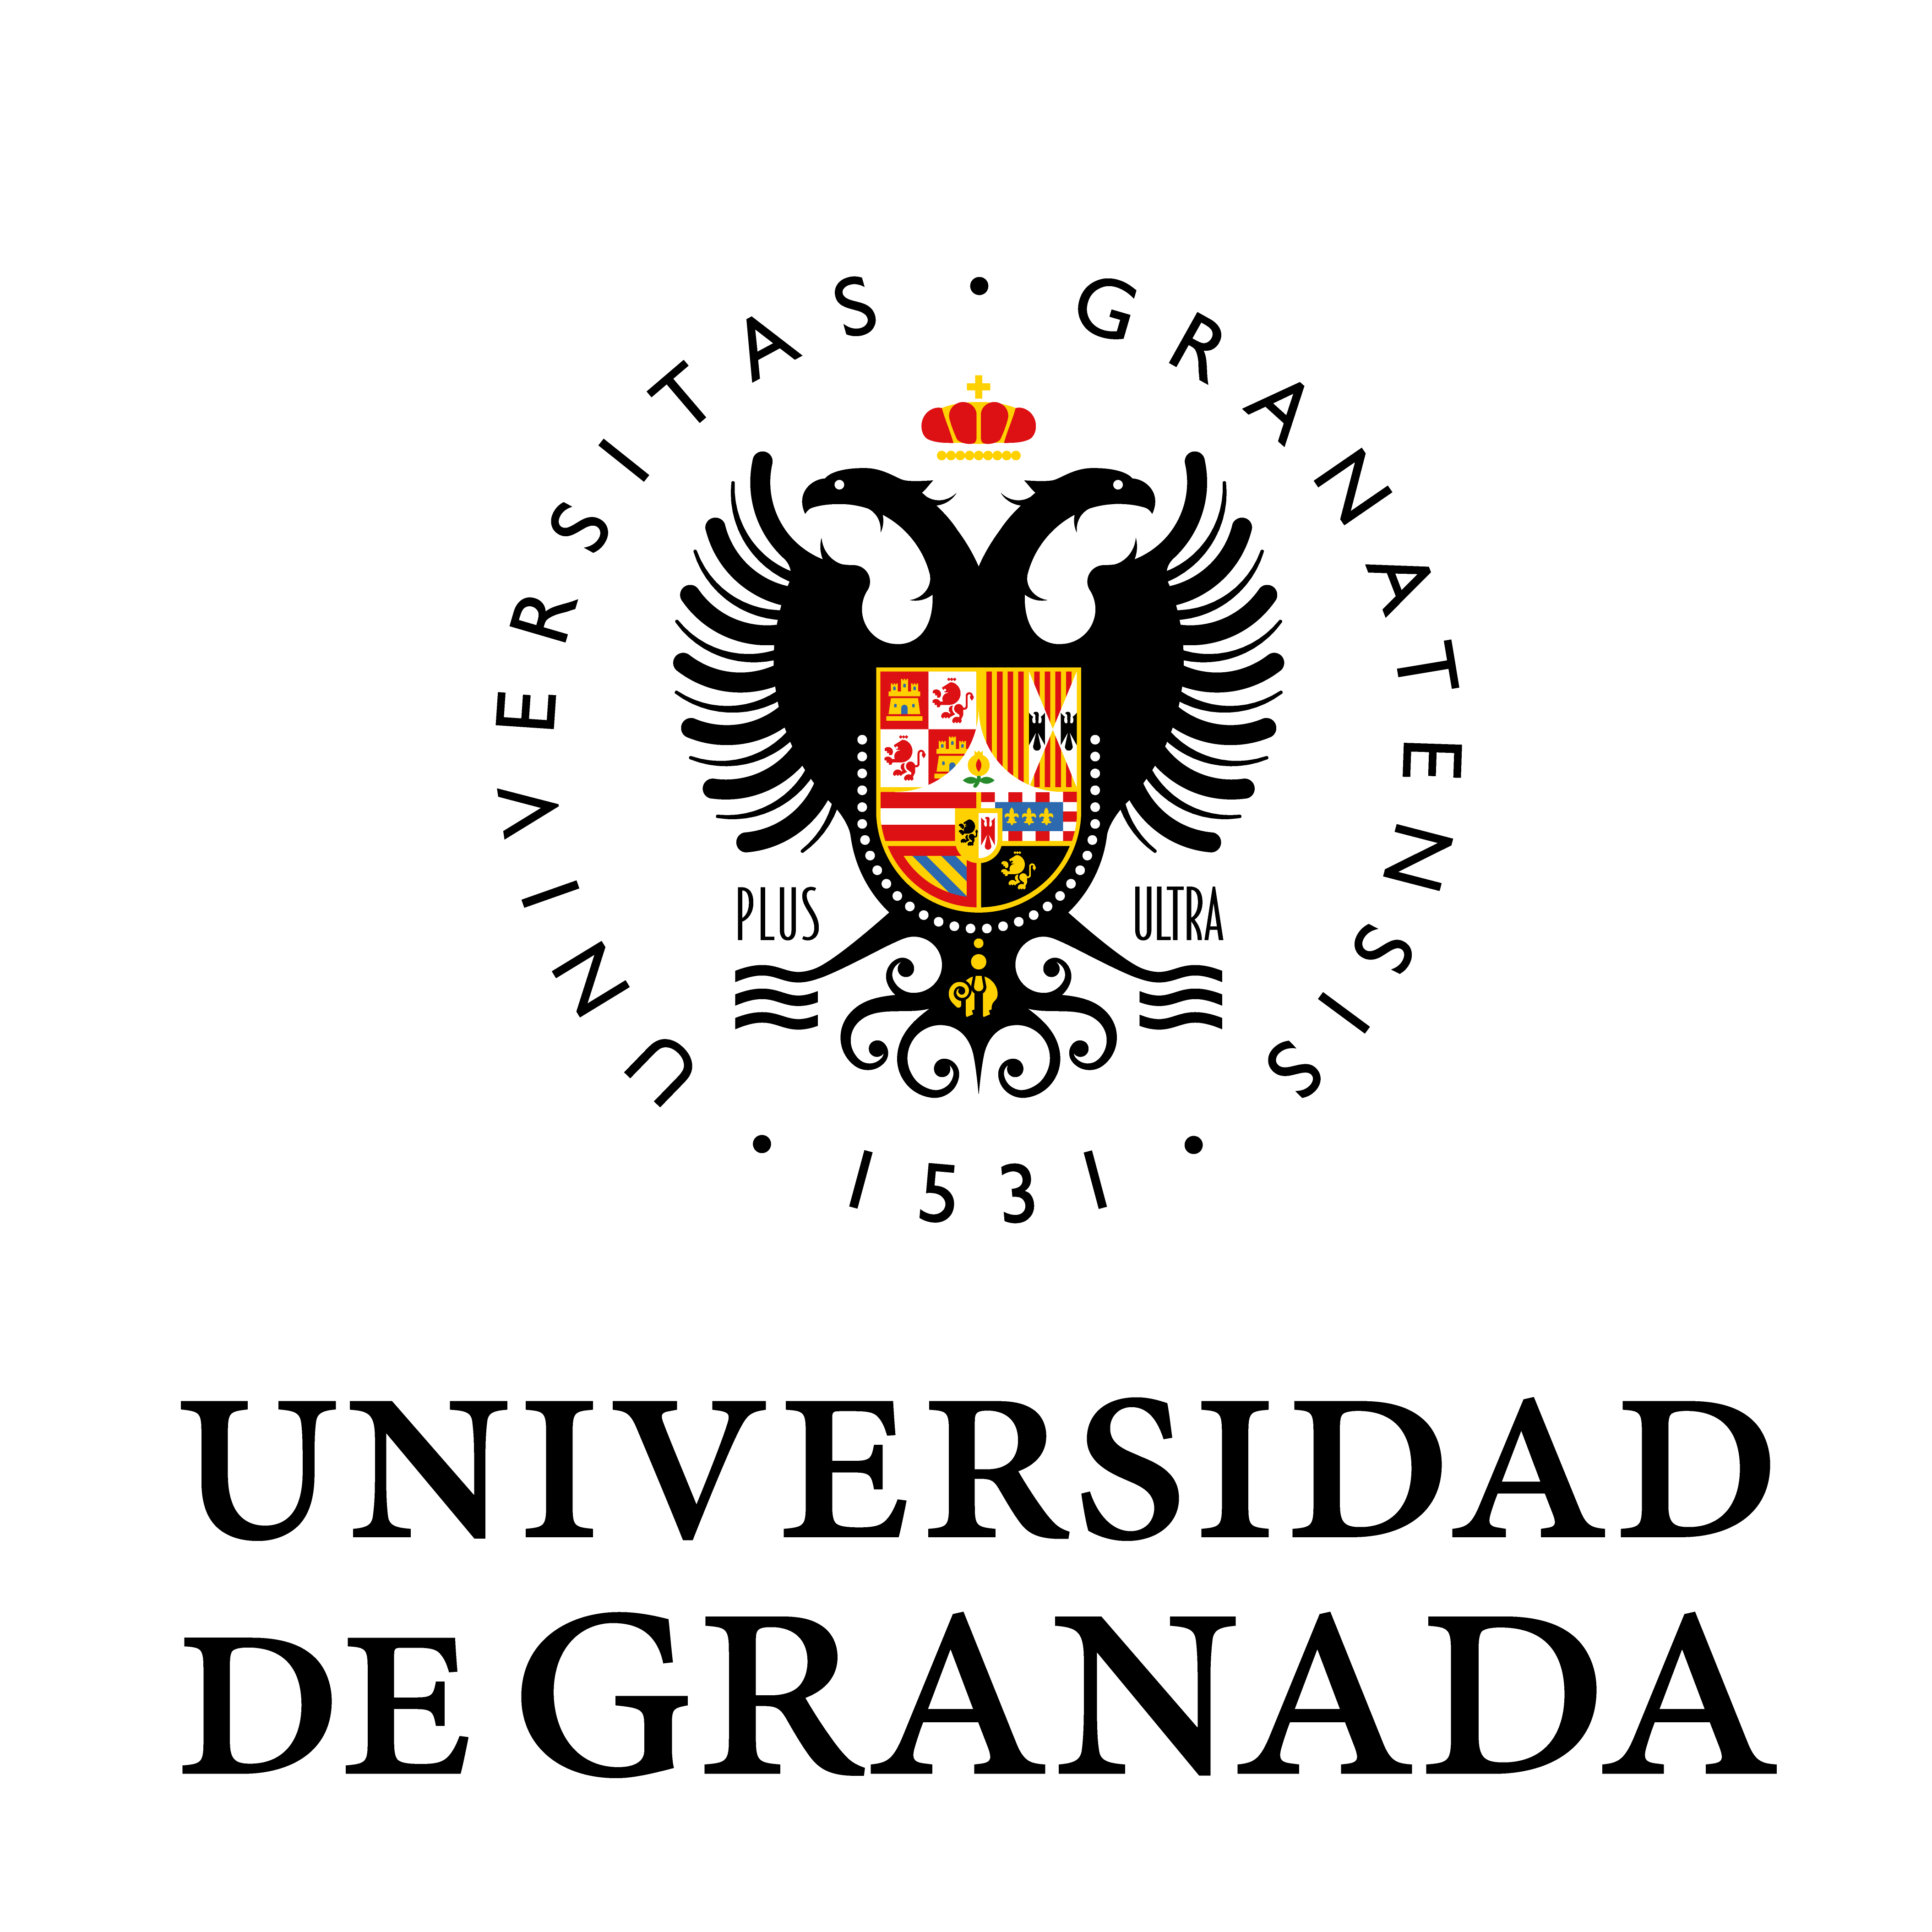
\includegraphics[scale = 0.50]{ugr.png}\\[0.7 cm]
    %\textsc{\LARGE Universidad de Granada}\\[2.0 cm]   
    \textsc{\large 3º CSI 2019/20 - Grupo 1}\\[0.5 cm]            
    \textsc{\large Grado en Ingeniería Informática}\\[0.5 cm]              
    \rule{\linewidth}{0.2 mm} \\[0.2 cm]
    { \huge \bfseries \thetitle}\\
    \rule{\linewidth}{0.2 mm} \\[1 cm]
    
    \begin{minipage}{0.4\textwidth}
        \begin{flushleft} \large
            \emph{Autor:}\\
            \theauthor\\ 
			 \emph{DNI:}\\
            77021623-M
            \end{flushleft}
            \end{minipage}~
            \begin{minipage}{0.4\textwidth}
            \begin{flushright} \large
            \emph{Asignatura: \\
            Técnicas de los Sistemas Inteligentes}   \\     
            \emph{Correo:}\\
            advy99@correo.ugr.es           
        \end{flushright}
    \end{minipage}\\[0.5cm]
  
    {\large \thedate}\\[0.5cm]
    %{\url{https://github.com/advy99/TSI/}}
    {\doclicenseThis}
 	
    \vfill
    
\end{titlepage}

%%%%%%%%%%%%%%%%%%%%%%%%%%%%%%%%%%%%%%%%%%%%%%%%%%%%%%%%%%%%%%%%%%%%%%%%%%%%%%%%%%%%%%%%%

%\tableofcontents
%\pagebreak

%%%%%%%%%%%%%%%%%%%%%%%%%%%%%%%%%%%%%%%%%%%%%%%%%%%%%%%%%%%%%%%%%%%%%%%%%%%%%%%%%%%%%%%%%

\section{Introducción}

Para esta práctica se nos pide desarrollar un agente que juegue al juego \"Boulder Dash\", videojuego de 1984 para las computadores Atari. Simularemos este juego a través del entorno de desarrollo GVGAI, desarrollado en Java. Este entorno de desarrollo se caracteriza por ser una IA que juega a juegos genéricos, donde el objetivo es conseguir ciertos materiales, y cuando se obtengan dichos materiales salir por una puerta, todo esto evitando enemigos (si los hubiera). El juego en el que nos centraremos, ``Boulderdash'', tiene el mismo objetivo aunque para el desarrollo de la práctica se nos plantean algunas variaciones que veremos más adelante.

El juego se desarrolla en un mapa cuadriculado para nuestro personaje (más adelante veremos que los enemigos tienen una forma distinta de moverse). Los movimientos posibles serán moverse hacia arriba, abajo, izquierda y derecha. Además de esta acciones, si el personaje tiene que girarse, utilizará una acción para esto, es decir, si esta mirando hacia la derecha y quiere ir a la izquierda, necesitará dos ordenes de moverse a la izquierda, una para girarse y otra para realizar el movimiento.

Nuestro agente tendrá un segundo inicial para realizar cálculos a modo de preparación', tras eso, deberá responder con una de estas acciones en menos de 40ms, si tarda entre 40ms y 50ms automáticamente responderá con la acción de no hacer nada, y en caso de tardar más de 50ms el agente quedará descalificado y perderá.

El juego finaliza cuando se consigue el objetivo (en el caso del comportamiento deliberativo) o cuando el personaje sobrevive 2000 acciones (ticks dentro del juego, en el caso del comportamiento reactivo).

En este documento explicaré las consideraciones tomadas al desarrollar la práctica, y la forma en la que ha ido evolucionando el código desde el nivel 1 hasta el nivel 5.

\subsubsection{Consideraciones previas}

Para el desarrollo del agente suponemos que siempre hay un portal de salida en los mapas que requieran comportamiento deliberativo, además el portal escogido para salir ha de ser único y accesible. Si no es único (existe más de un portal), es seleccionado el más cercano al jugador en el momento de inicio del juego.

\section{Comportamiento deliberativo}

En el desarrollo de este apartado desarrollaremos el funcionamiento del agente deliberativo, es decir, el agente, con conocimiento del entorno, buscará la mejor forma de llegar al objetivo, en este nivel la puerta.

De cara a conseguir esto he decidido implementar el algoritmo de búsqueda de caminos A*, este algoritmo combina el algoritmo de Dijkstra con el algoritmo greedy Best-First, añadiendo el componente de heurística con el que guiaremos la búsqueda intentando avanzar hacia la solución, en lugar de explorar de forma uniforme el espacio de búsqueda.

Dicho esto, A* evaluará los nodos de la siguiente forma:

$$ f(n) = g(n) + h(h) $$

Donde $g(n)$ es el coste desde el punto de partida hasta el nodo $n$ y $h(n)$ es la heurística, es decir, la estimación que hacemos del coste desde el nodo $n$ hasta el nodo objetivo.

He escogido este algoritmo ya que cumple las dos restricciones básicas para que este funcione:

\begin{enumerate}
	\item El grafo es localmente finito: Para cada nodo el número de hijos es finito. Esto se cumple ya que cada nodo tendrá 4 hijos (cada una de las acciones, a excepción de quedarse quieto, ya que ese hijo es el propio nodo y no es necesario explorarlo).
	\item El coste de pasar de un nodo cualquiera a uno de sus sucesores es estrictamente positivo.
\end{enumerate}

No solo he escogido el algoritmo A* por estas características, que simplemente me permiten implementarlo en nuestro problema, si no porque como explicaré más adelante, para nuestro problema A* será un algoritmo completo, admisible, y con una heurística consistente (continua) lo que nos reducirá el coste computacional del algoritmo.

\subsubsection{Completitud de A*}

Para poder asegurar que A* es completo basta con demostrar que el grafo es finito, es decir, tiene un número finito de caminos acíclicos. En nuestro caso esto se cumple, ya que el número de casillas del mapa es finito, tendremos un número finito de caminos y podemos asegurar la completitud del algoritmo.

\subsubsection{Admisibilidad de A*}

En este caso la admisibilidad de A* depende de la heurística usada, ya que influirá en el orden de exploración de los nodos. Para que A* sea admisible, la heurística usada debe ser admisible, es decir, que se cumpla $h(n) \leq h^*(n)$. Básicamente que la estimación de nuestra heurística no sobreestime el coste real de llegar al nodo objetivo.

En esta práctica, al ser un mundo cuadriculado usaré como heurística la distancia Manhattan, en la que una casilla tendrá un coste de uno. Esta heurística es admisible ya que cualquier movimiento, como mínimo, tendrá coste uno, por lo que nuestra estimación será igual o menor al coste real, en el mejor de los casos (linea recta) $h(n) = h^*(n)$, y en caso de que tenga que hacer algún giro $h(n) = h^*(n) - num\_giros$, por lo que la heurística siempre es admisible, y en caso de encontrar algún obstáculo necesitará gastar más ticks para llegar al objetivo, luego será admisible en todos los casos.

\subsubsection{Heurística consistente (continua)}

A* usando distancia Manhattan como heurística tiene la ventaja de que es consistente, es decir, para cada nodo $n$ y cada sucesor $n'$ generado a parir de $n$ tras cualquier acción $a$, el coste estimado de alcanzar el objetivo desde $n$ es menor o igual que el coste de alcanzar $n'$ más el coste estimado de alcanzar el objetivo desde $n'$, es decir:

$$ h(n) \leq c(n, a, n') + h(n') $$

Esta desigualdad triangular, cumplida si usamos la distancia Manhattan, nos asegura que cuando el algoritmo explora (abre) un nodo, este va a ser el mejor camino encontrado para llegar a ese nodo, por lo que una vez que un nodo entra en cerrados, sabemos que ese es el mejor camino para ese nodo, haciendo que si encontramos otro camino a dicho nodo simplemente los desechamos porque esta propiedad nos asegura que va a ser un peor camino.


\subsubsection{Decisión de la elección del algoritmo}

Una vez explicado el funcionamiento de A*, en este apartado procederé a explicar porque finalmente he escogido dicho algoritmo frente a otros algoritmos de búsqueda de caminos. He decidido explicarlo en este orden para que se entiendan las propiedades por las que A* es una mejor opción.

\textbf{IDA*}: A pesar de que el algoritmo IDA* puede parecer una buena idea, ya que seguimos manteniendo las propiedades antes comentadas por el A* con la ventaja de que no tenemos que almacenar información sobre los nodos frontera por explorar como en el algoritmo escogido, si no que solo almacena información sobre el camino actual, la forma de conseguir esta mejora en memoria hace que el algoritmo no sea viable en tiempo, ya que ha de ir explorando rama a rama todos los posibles caminos.

Al tener tan solo 40ms para realizar los distintos cálculos, sumado a que en nuestro caso no existirá el problema de memoria al ser mapas pequeños y ahorrarnos la reexploración al usar una heurística consistente he decidido no usar este algoritmo ya que la única ventaja que nos ofrece no es realmente necesaria, sumado a la perdida de tiempo de computo y posiblemente la descalificación por no encontrar solución a tiempo.

\textbf{Algoritmo de Dijkstra}: Este algoritmo proporciona el camino más corto entre un nodo y todos los demás, por lo que no es factible para grafos grandes, además, este algoritmo no usa búsqueda heurística, sumado a que el algoritmo A* es una variación de este algoritmo, que mejora la búsqueda al hacer uso de la heurística, escogería este algoritmo si no existiera heurística que me garantice que A* es admisible, pero como hemos comentado antes, existe y además mejora el algoritmo al ser consistente.

\textbf{Algoritmo Greedy Best-First Search}: Este algoritmo usa únicamente la información heurística, por lo que busca el camino más directo al destino, pero sin tener en cuenta lo ya recorrido, por lo que un camino que parecía una buena opción al puede ser un mal camino al no tener en cuenta el coste hasta ese momento.

De nuevo, el algoritmo escogido es una combinación de este algoritmo Greedy y el algoritmo del apartado anterior, de forma que tenga en cuenta la estimación del camino, pero siendo consciente de lo que ya lleva recorrido, y cambiando de camino si es necesario.


\textbf{Otros algoritmos}: También he tenido en cuenta otros algoritmos, como el algoritmo de búsqueda por franjas o el algoritmo Theta* visto en teoría, sin embargo me he encontrado que son modificaciones de IDA* o A* para casos concretos en los que A* no se comporta bien, sin embargo en nuestro problema no es el caso, así que he decidido no implementarlos.

\subsection{Deliberativo simple}

De cara al desarrollo del agente deliberativo simple he hecho uso del algoritmo A* con heurística distancia Manhattan como antes he comentado. En este nivel nuestro agente simplemente intenta encontrar la puerta y salir.

\subsubsection{Implementación del algoritmo A*}

Para implementar el algoritmo A* he usado la clase \texttt{Node} disponible en el paquete \texttt{pathfinder} de GVGAI, aunque realizando algunas modificaciones:

\begin{enumerate}
	\item Añadido variable para la orientación, la cual tenemos en cuenta para comprobar si dos nodos son iguales.
	\item Modificación del método \texttt{getMov} para que en lugar de no devolver nada (el uso era interno) devuelva la acción que ha conseguido llegar a ese estado.
\end{enumerate}

El primer punto es bastante importante, ya que si no sería mucho más difícil tener en cuenta la orientación al generar los nodos hijos, como veremos más adelante, lo que nos llevaría a un calculo erróneo de $g(n)$. Con respecto a la representación de la orientación, he usado 0, 1, 2 y 3, que representan arriba, derecha, abajo e izquierda respectivamente, ya que la representación usada por GVGAI me parecía demasiado compleja para el problema que tratamos.

También he implementado una función para pasar de la representación de orientación dada por GVGAI a la mía, disponible en el código fuente que acompaña esta memoria.

El segundo punto es importante ya que usaremos ese método para obtener la lista de movimientos una vez tengamos la solución.

Dicho esto, la implementación del algoritmo podemos consultarla en el fichero \texttt{Agent.java}. La implementación usa colas con prioridad para gestionar abiertos y cerrados, y simplemente va generando los hijos del mejor de abiertos, si un hijo no se ha generado nunca, lo inserta en abiertos, si un hijo ya se ha generado y está en abiertos nos quedamos con el hijo de menor coste, y si generamos un hijo que ya está en cerrados directamente lo desechamos, ya que al usar una heurística consistente sabemos que el que está en cerrados ya es el mejor camino. Este algoritmo devolverá el nodo solución. Una vez tenemos dicho nodo solución, simplemente lo recorremos hasta que su padre sea nulo, metiendo las acciones recogidas con el método \texttt{getMov}, en caso de que sea la acción nula duplicamos la acción del tope de la pila, ya que la acción nula equivale a quedarse en la misma casilla, lo que indica que estamos girando.

\subsubsection{Cambios necesarios en el método act y constructor del agente}

Los cambios que he tenido que realizar en el constructor son crear una variable de tipo Pila que almacenará los pasos necesarios para llegar al destino. He escogido este tipo de estructura de datos ya que siempre accederemos al elemento superior, y aunque a primera vista de la impresión de que estamos accediendo en orden inverso a los elementos, nuestro A* nos devolverá el nodo solución, y para obtener el camino iremos desde dicho nodo hacia el inicial a través del atributo \texttt{parent} de los distintos nodos, por lo que estamos leyendo en orden inverso el camino. Al almacenarlo en una pila, lo almacenamos en orden inverso al leído, es decir, el orden correcto.

Los cambios necesarios en el método \texttt{act} han sido añadir una condición, si el plan esta vacío, lanzamos el algoritmo A* y calculamos el plan a partir del nodo devuelto. En este caso suponemos que siempre existe el camino, es decir, que siempre hay portal (condición necesaria de la práctica). Si el plan no está vacío simplemente sacamos acciones del plan y las devolvemos.

Como hemos comprobado en la explicación del algoritmo, tenemos un algoritmo completo, admisible, consistente y además con unos tiempos de ejecución muy buenos.



Esta implementación nos hace obtener 27 ticks en el mapa 5

\textbf{Importante:} Además de modificar el fichero \texttt{boulderdash.txt} para establecer el límite de gemas a -1, también tenemos que modificar la primera linea del constructor del agente, estableciendo \texttt{gemas\_a\_obtener = 0}.

\subsection{Deliberativo compuesto}

En este nivel, además de alcanzar la salida, el objetivo será conseguir 10 gemas distribuidas por el mapa. Para conseguir esto simplemente pruebo los distintos caminos posibles entre las gemas, es decir, suponiendo que tenemos 3 gemas A, B y C probaremos con los caminos: \{A, B, C\}, escogeremos el de menor distancia y generamos sus hijos, por ejemplo, suponiendo que B tiene menor distancia tendríamos: \{A, C, BA, BC\}, y volveríamos a coger el de menor distancia, hasta que lleguemos al objetivo, coger las 10 gemas, cuando lleguemos obtener todas y saquemos ese camino, por ejemplo el \{BAC\}, todavía tenemos que introducir en la lista de caminos el \{BACP\}, para comprobar que con la vuelta al portal es el mejor camino. Para realizar la implementación tenemos que tener algunas cosas más en cuenta.

Para empezar, el coste de realizar este calculo es exponencial, en el ejemplo anterior, con 3 gemas, tenemos 3! + 3! posibles caminos (3! por las combinaciones A, B y C y otro 3! por dichas combinaciones sumarles el portal para llegar a la salida).

Para seleccionar los nodos uso la estrategia del algoritmo de Dijkstra, el que tenga menor coste. El coste será la distancia entre las distintas gemas, el inicio, en nuestro ejemplo \{A, B, C\}, cada gema tendrá asociada el coste de ir desde la posición del jugador hasta A, hasta B o hasta C respectivamente. Para calcular estas distancias usaremos el algoritmo A*, ya que sabemos que con el obtenemos el optimo. Al principio del calculo relleno la parte superior de una matriz con tantas filas y columnas como número de gemas más dos (este último más dos para la distancia del punto inicial a las gemas y la distancia de las gemas al portal).

He pensado en como mejorar este algoritmo, pero tras darle muchas vueltas no se me ocurre ninguna heurística que funcione a la hora de escoger que camino puede ser mejor que otro, ya que todas las que he probado (distancia entre una secuencia aleatoria de entre las gemas restantes, distancia de la última gema al portal multiplicado por el número de gemas restantes, distancia más grande de la matriz por número restante de gemas, entre otras) me daban peores resultados que un greedy simple, por lo que simplemente he dejado el algoritmo de esta forma, ya que con el segundo del constructor es capaz de calcularlo en todos los mapas que he probado, pero con una condición. Esta condición es que tenga menos de 12 gemas, si el mapa tiene 15, el límite superior con el que se corrige, tarda demasiado.

Esto lo he solucionado usando solo las doce gemas más cercanas al jugador (usando \texttt{getResourcePositions()}), ya que podemos suponer que esas gemas son las más prometedoras.

Con esto nos aseguramos obtener buenos resultados, que aunque no sean el óptimo, estarán muy cerca, porque será el óptimo de entre esas 12 gemas. En caso de que el mapa tenga menos de 12 gemas, obtendremos el óptimo, como por ejemplo en el mapa 6, que obtenemos 84 ticks.

\section{Comportamiento reactivo}

El comportamiento reactivo se basa en evitar los enemigos que encontramos por el mapa. Para el desarrollo de este comportamiento tendré un mapa de calor, que me indicará las zonas peligrosas del juego. En este caso el agente actuará de la forma más simple posible: moverse a la casilla de menor riesgo inmediata al personaje. He decidido seguir la navaja de Ockham, la forma más simple suele ser la más probable, en este caso, la forma que mejor funcione, he decidido esto tras varios intentos de buscar la mejor forma de moverse por el mapa, sin conseguir claramente un vencedor, a excepción del método, que con un mapa de calor detallado y preciso se comporta muy bien (con las pruebas realizadas siempre sobrevive el agente, a excepción de casos extremos como pasillos).

\subsection{Reactivo simple}

De cara a implementar el agente reactivo simple he diseñado una matriz a modo de mapa de calor. Tendremos dos matrices: \texttt{mapa\_base} y \texttt{mapa\_calor}. El mapa base lo calcularemos únicamente una vez en el constructor del agente, y contendrá información del peligro de objetos fijos (muros), que nunca cambiarán durante la ejecución. El mapa de calor contendrá el mapa de calor durante esa iteración, y será el que calcularemos cada vez que se ejecuta el método \texttt{act}.

La forma de calcular el mapa base es muy simple, inicializado a 0.0, recorremos todos los muros, y en todas las casillas alrededor del muro, con radio 2, le sumamos 1.0 si la distancia es de 1, o 0.5 si la distancia es de 2. En esta distancia tenemos en cuenta las diagonales, ya que los enemigos en realidad no se mueven en grid, si no por píxeles, por lo que un enemigo en un tick podría moverse en diagonal, así que la casilla diagonal tiene el mismo peligro que las perpendiculares. La propia posición del muro la pondremos a más infinito, para que el personaje nunca intente ir hacia ella. Por lo tanto, el mapa para un muro quedaría de la siguiente forma:

\vspace{-0.4cm}

\begin{table}[H]
\centering

\begin{tabular}{lllll}
0.5 & 0.5 & 0.5 & 0.5 & 0.5                     \\
0.5 & 1.0 & 1.0 & 1.0 & 0.5                     \\
0.5 & 1.0 & Inf    & 1.0 & 0.5                     \\
0.5 & 1.0 & 1.0 & 1.0 & 0.5                     \\
0.5 & 0.5 & 0.5 & 0.5 & \multicolumn{1}{c}{0.5}
\end{tabular}
\end{table}

\vspace{-0.5cm}

De forma que en el caso extremo en el que tengamos una posición totalmente rodeada de muros, su valor de riesgo será 16. Con este criterio (y de cara al comportamiento reactivo compuesto, como explicaré más adelante) en cada ejecución de \texttt{act} completaremos el mapa de peligro de esa ejecución teniendo en cuenta tanto los enemigos como las gemas.


En el caso de los enemigos tendremos un radio bastante mayor, de 5, ya que si mantenemos el radio de 2 o incluso 3 nos arriesgamos a que tengamos que girar y el enemigo se acerque demasiado. Como he comentado, como el valor máximo que puede generar los muros es 16, el valor más pequeño sumado por un enemigo es 17, de esta forma podemos distinguir si estamos en riesgo por un enemigo o por un muro, además del sentido lógico, ya que los enemigos son un peligro mucho mayor a los muros. Realizaremos de la misma forma que antes el mapa de calor, pero sumando 17, 20, 25, 30 o 35 si el radio es 5, 4, 3, 2 o 1 respectivamente. De nuevo la casilla del enemigo le daremos un valor de infinito, para evitar movernos a esa posición.

Para las gemas realizaremos la misma operación que con los muros, pero en lugar de sumar al mapa de peligro, restaremos peligro, permitiendo moverse entre algún enemigo (si nos fijamos en el código, solo cerca del primer o segundo nivel de peligro, nunca dentro de un rango superior a 3 casillas) para coger una gema.

En todo nivel que no existan gemas, o el número de gemas sea menor que 10, supondremos que siempre hay riesgo. La forma de moverse con riesgo, como ya hemos comentado, es moverse a la casilla de al rededor con menor riesgo.

En un mapa que siempre hay riesgo (de momento tanto en el reactivo simple como el compuesto siempre lo hay) he añadido que en las zonas centrales tenga menos riesgo, intentando evitar los bordes del mapa. En caso de que en el centro existan muros, estos se compensarán con el peligro que ya les dimos anteriormente.


\subsection{Reactivo compuesto}

Para el reactivo compuesto la forma de trabajar es exactamente la misma, la única diferencia es al asignar el mapa de peligro de los enemigos, he modificado la forma de asignación del peligro para que en zonas donde afecte el peligro de dos enemigos, solo tenga en cuenta el de uno (el que tenga mayor peligro), de forma que si dos enemigos le encierran contra una pared, tenga la posibilidad de pasar entre los dos enemigos antes de acercarse a una esquina en la que la probabilidad de morir es más alta.

Tanto en el reactivo simple como en el reactivo compuesto esto me ha funcionado bastante bien, ganando en casi todas las partidas que he ejecutado (en mapas con muchos muros y pasillos si es más probable que muera por la complejidad del mapa), tanto el simple como en el compuesto, probando con distintos mapas (mapa en blanco, con muros por el mapa, mapas con pasillos, etc)

\section{Comportamiento reactivo-deliverativo}

El desarrollo de este modo ha sido simple, en el método \texttt{act} he introducido variables booleanas que controlan el flujo del agente como si fuera una máquina de estados, en el caso de no tener gemas, se comportará de forma reactiva, en el caso de tener gemas, comprobará si existe riesgo, y en caso de no existir riesgo se comportará de forma deliberativa, como en el nivel 3 y 4 siempre hay riesgo, no tenemos problemas. En el nivel 2, al tener las gemas, aunque los muros añaden riesgo, está por debajo del umbral considerado para comenzar a actuar con riesgo, por lo que siempre se comportará de forma deliberativa. El único caso especial es el nivel 1, en el que tenemos que modificar el juego para establecer el límite de gemas a -1, y en nuestro agente cambiar la variable \texttt{gemas\_a\_obtener} a 0.

De esta forma para este nivel continuará su ejecución de forma deliberativa buscando las gemas, a excepción de si entra en el rango de un enemigo, que se comenzará a mover de forma reactiva. Cuando sale del rango y vuelve a actuar de forma deliberativa, vuelve a recalcular el camino para la gema que estaba buscando, y en el caso de que nos queden menos de 6 gemas, recalcularemos el camino (menos de 6 ya que el método de calcular el camino es costoso, así que he decidido no arriesgarme a quedarme sin tiempo).

\section{Resultados}

Resultados con los mapas dados (he probado con otros mapas, pero no dispongo de espacio para mostrarlos ni mostrar su solución):

\begin{table}[H]
\centering
\begin{tabular}{|c|c|c|c|c|c|}
\hline
                         & \textbf{Mapa 5} & \textbf{Mapa 6} & \textbf{Mapa 7} & \textbf{Mapa 8} & \textbf{Mapa 9} \\ \hline
\textbf{Ticks/sobrevive} & 27              & 84              & Sobrevive       & Sobrevive       & 128,6 (media)            \\ \hline
\end{tabular}
\end{table}

\textbf{Aviso:} Los ticks en el mapa 9 son de media tras 10 ejecuciones, en ocasiones obtenemos unos 84, mientras que en otras hemos llegado a 250. Las ejecuciones de los mapas 7 y 8 también, de unas 10 ejecuciones cada uno solo ha muerto una vez en el compuesto.

\section{Material consultado para realizar la práctica}

Apuntes y diapositivas de teoría, prácticas y el libro ``Inteligencia Artificial: Un enfoque moderno'' de Stuart Russell y Peter Norvig.

\end{document}
